\documentclass{beamer}

\mode<presentation> {

%\usetheme{default}
%\usetheme{AnnArbor}
%\usetheme{Antibes}
%\usetheme{Bergen}
%\usetheme{Berkeley}
%\usetheme{Berlin}
%\usetheme{Boadilla}
%\usetheme{CambridgeUS}
%\usetheme{Copenhagen}
%\usetheme{Darmstadt}
%\usetheme{Dresden}
%\usetheme{Frankfurt}
%\usetheme{Goettingen}
%\usetheme{Hannover}
%\usetheme{Ilmenau}
%\usetheme{JuanLesPins}
%\usetheme{Luebeck}
\usetheme{Madrid}
%\usetheme{Malmoe}
%\usetheme{Marburg}
%\usetheme{Montpellier}
%\usetheme{PaloAlto}
%\usetheme{Pittsburgh}
%\usetheme{Rochester}
%\usetheme{Singapore}
%\usetheme{Szeged}
%\usetheme{Warsaw}


%\usecolortheme{albatross}
%\usecolortheme{beaver}
%\usecolortheme{beetle}
%\usecolortheme{crane}
%\usecolortheme{dolphin}
%\usecolortheme{dove}
%\usecolortheme{fly}
%\usecolortheme{lily}
%\usecolortheme{orchid}
%\usecolortheme{rose}
%\usecolortheme{seagull}
%\usecolortheme{seahorse}
%\usecolortheme{whale}
%\usecolortheme{wolverine}

%\setbeamertemplate{footline} % To remove the footer line in all slides uncomment this line
%\setbeamertemplate{footline}[page number] % To replace the footer line in all slides with a simple slide count uncomment this line

%\setbeamertemplate{navigation symbols}{} % To remove the navigation symbols from the bottom of all slides uncomment this line
}

\usepackage{graphicx} % Allows including images
\usepackage{booktabs} % Allows the use of \toprule, \midrule and \bottomrule in tables
\usepackage{amsfonts}
\usepackage{mathrsfs, bbold}
\usepackage{amsmath,amssymb,graphicx}
\usepackage{mathtools} % gather
\usepackage[export]{adjustbox} % right-aligned graphics

%----------------------------------------------------------------------------------------
%	TITLE PAGE
%----------------------------------------------------------------------------------------

\title["10"]{10: Introduction to Bayesian Computation}

\author{Taylor} 
\institute[UVA] 
{
University of Virginia \\
\medskip
\textit{} 
}
\date{} 

\begin{document}
%----------------------------------------------------------------------------------------

\begin{frame}
\titlepage 
\end{frame}

%----------------------------------------------------------------------------------------
\begin{frame}
\frametitle{Introduction}

This chapter gives an overview for how to approximate intractable quantities such as posterior expectations and predictions. 

\end{frame}

%----------------------------------------------------------------------------------------
\begin{frame}
\frametitle{Definitions}

{\bf Numerical integration} methods approximate integrals. 
\newline

These methods can be loosely categorized as either {\bf stochastic} or {\bf deterministic} (e.g. quadrature methods).


\end{frame}




%----------------------------------------------------------------------------------------
\begin{frame}
\frametitle{Deterministic Methods}

{\bf Deterministic methods} don't draw samples, and instead approximate the integral by summing up approximate volumes:
\[
E[h(\theta) \mid y] = \int h(\theta) p(\theta \mid y) \text{d}\theta \approx \frac{1}{S} \sum_{s=1}^S w_s h(\theta^s)p(\theta^s \mid y)
\]

\end{frame}

%----------------------------------------------------------------------------------------
\begin{frame}
\frametitle{Stochastic Methods}

{\bf Stochastic methods} involve sample averages of simulated draws from some distribution. There are many ways to do this, but generally
\[
E[h(\theta) \mid y] = \int h(\theta) p(\theta \mid y) \text{d}\theta \approx \frac{1}{S} \sum_{s=1}^S h(\theta^s)
\]
with $\theta^s \sim p(\theta \mid y)$, or
\[
E[h(\tilde{y}) \mid y] = \int h(\tilde{y}) p(\tilde{y} \mid y) \text{d} \tilde{y} \approx \frac{1}{S} \sum_{s=1}^S h(\tilde{y}^s)
\]
with $\tilde{y} \sim p(\tilde{y} \mid y)$

\end{frame}

%----------------------------------------------------------------------------------------
\begin{frame}
\frametitle{Stochastic Methods}

Drawing $\tilde{y}$ samples can be done in a two-stage way:
\begin{enumerate}
\item draw $\theta^s \sim p(\theta \mid y)$
\item draw $\tilde{y}^s \sim p(\tilde{y} \mid \theta^s)$
\end{enumerate}
\pause

If it's available, you should probably use a Rao-Blackwellized procedure, though:
\[
E[h(\tilde{y}) \mid y] = E[E\left( h(\tilde{y}) \mid \theta \right) \mid y] \approx \frac{1}{S} \sum_{s=1}^S E\left( h(\tilde{y}) \mid \theta^s \right)
\]
with $\theta^s \sim p(\theta \mid y)$


\end{frame}
%----------------------------------------------------------------------------------------
\begin{frame}[fragile]
\frametitle{Approximating the posterior on a grid}

We used this method earlier for the rat tumor example!
\newline

Given that we can evaluate the unnormalized target $p(\theta, y) = p(y \mid \theta)p(\theta)$, we choose a nonrandom grid of points (think \verb|seq|) $\theta_1, \ldots, \theta_S$, and then we approximate the the continuous posterior with a discrete random variable with pmf equal to
\[
\tilde{p}(\theta_j \mid y) = \frac{p(y \mid \theta_j)p(\theta_j)}{\sum_{s=1}^S p(y \mid \theta_s)p(\theta_s) }
\]
for any $\theta_j \in \{\theta_1, \ldots, \theta_s\}$

\end{frame}

%----------------------------------------------------------------------------------------
\begin{frame}[fragile]
\frametitle{Approximating the posterior on a grid}

From now on we will write the posterior in terms of an unnormalized density $q(\theta \mid y)$. In other words:
\[
p(\theta \mid y) = \frac{q(\theta \mid y)}{ \int q(\theta \mid y) \text{d}\theta}
\]

Most (maybe all) of the sampling techniques will assume that we can't evaluate $p(\theta \mid y)$, but that we can evaluate $q(\theta \mid y)$

\end{frame}
%----------------------------------------------------------------------------------------
\begin{frame}[fragile]
\frametitle{Rejection Sampling aka Accept-Reject sampling}

Setup
\begin{enumerate}
\item $p(\theta \mid y)$ the target, posterior
\item $q(\theta \mid y) = p(y \mid \theta) p(\theta)$ the unnormalized target
\item $g(\theta)$ the ``instrumental" or ``proposal" distribution
\item need $q(\theta \mid y) / g(\theta) \le M$ uniformly
\item $g \gg q$ the proposal ``dominates" your target (won't divide by $0$)
\end{enumerate}
We are free to choose our own $g(\theta)$. For the time being, we assume that $\int g(\theta) \text{d}\theta = 1$.

\end{frame}
%----------------------------------------------------------------------------------------
\begin{frame}[fragile]
\frametitle{Rejection Sampling aka Accept-Reject sampling}


To (potentially) produce one draw:
\begin{enumerate}
\item propose the draw $\theta^s \sim g(\theta)$
\item draw $U \sim \text{Uniform}(0,1]$
\item accept $\theta^s$ if $U < q(\theta^s \mid y) / \{ q(\theta^s)  M\}$
\end{enumerate}


\end{frame}
%----------------------------------------------------------------------------------------
\begin{frame}[fragile]
\frametitle{Rejection Sampling aka Accept-Reject sampling}
\begin{align*}
P\left( \theta \le t \bigg\rvert U \le \frac{q(\theta \mid y)}{M g(\theta) } \right) 
&= \frac{P\left( \theta \le t , U \le \frac{q(\theta \mid y)}{M g(\theta) } \right)}{P\left(U \le \frac{q(\theta \mid y)}{M g(\theta) } \right)} \\
&= \frac{\int_{-\infty}^t \int_0^{ \frac{q(\theta \mid y)}{M g(\theta) } }g(\theta)1 \text{d}u \text{d}\theta }{ \int_{-\infty}^{\infty} \int_0^{ \frac{q(\theta \mid y)}{M g(\theta) } }g(\theta)1 \text{d}u \text{d}\theta } \\
&= \frac{\int_{-\infty}^t g(\theta)\frac{q(\theta \mid y)}{M g(\theta) }  \text{d}\theta }{ \int_{-\infty}^{\infty} g(\theta)  \frac{q(\theta \mid y)}{M g(\theta) } \text{d}\theta } \\
&= \frac{\int_{-\infty}^t q(\theta \mid y)  \text{d}\theta }{ \int_{-\infty}^{\infty}  q(\theta \mid y)\text{d}\theta } \\
&= p(\theta \le t \mid y).
\end{align*}
\end{frame}


%----------------------------------------------------------------------------------------
\begin{frame}[fragile]
\frametitle{Example 1}

Assume $y \sim \text{Normal}(\theta,1)$, and $p(\theta) = \frac{1}{\pi(1+\theta^2)}$. 
Our goal is to draw from
\begin{align*}
p(\theta \mid y) &\propto q(\theta\mid y) \\
&= p(y \mid \theta) p(\theta) \\
&= \frac{1}{\sqrt{2\pi}} \exp\left[-\frac{1}{2} (y-\theta)^2 \right] \frac{1}{\pi(1+\theta^2)} \\
&\propto \exp\left[-\frac{(\theta - y)^2}{2} - \log(1 + \theta^2) \right],
\end{align*}


\end{frame}

%----------------------------------------------------------------------------------------
\begin{frame}[fragile]
\frametitle{Example 1}

Let's assume that we want to use our prior distribution as a proposal: $g(\theta) = p(\theta)$. Then we have to find $M$:
\begin{align*}
\frac{q(\theta\mid y)}{g(\theta)} &= \frac{p(y \mid \theta) p(\theta)}{p(\theta)} \\
&= p(y \mid \theta) \\
&= \frac{1}{\sqrt{2\pi}} \exp\left[-\frac{1}{2} (y-\theta)^2 \right] \\
&\le \frac{1}{\sqrt{2\pi}} \overset{\text{def}}{=} M
\end{align*}

Our acceptance probability for draw $\theta^s$ is then
\[
q(\theta^s \mid y) / \{ q(\theta^s)  M\} = p(y \mid \theta^s) / M = \exp\left[-\frac{1}{2} (y-\theta^s)^2 \right]
\]


\end{frame}
%----------------------------------------------------------------------------------------
\begin{frame}[fragile]
\frametitle{Rejection Sampling aka Accept-Reject sampling}

Generally a good strategy is work with logarithms, and then exponentiate as late as possible.
\begin{verbatim}
y <- 2 # fake data
num_trials <- 1000
theta_proposals <- rt(num_trials, 1)
us <- runif(num_trials, min = 0, max = 1)
log_accept_prob <- function(theta){
  -.5*(y - theta)^2
}
probs <- exp(log_accept_prob(theta_proposals))
accepts <- ifelse(us < probs, TRUE, FALSE)
hist(theta_proposals[accepts]) # only the accepted draws
#hist(theta_proposals) # all draws!
\end{verbatim}

\end{frame}
%----------------------------------------------------------------------------------------
\begin{frame}[fragile]
\frametitle{Importance Sampling}

{\bf importance sampling} also involves ratios like the previous algorithm. However, instead of using those ratios to either accept or discard samples, it uses the ratios to weight samples. 
\newline

Pros: it runs in a nonrandom amount of time, and it doesn't require us to calculate an $M$. 
\newline
\pause

Setup
\begin{enumerate}
\item $p(\theta \mid y)$ the target, posterior
\item $q(\theta \mid y) = p(y \mid \theta) p(\theta)$ the unnormalized target
\item $g(\theta)$ the ``instrumental" or ``proposal" distribution
\item $g \gg q$ the proposal dominates your target 
\end{enumerate}
We are free to choose our own $g(\theta)$. For the time being, we assume that $\int g(\theta) \text{d}\theta = 1$.


\end{frame}
%----------------------------------------------------------------------------------------
\begin{frame}[fragile]
\frametitle{Importance Sampling}

Algorithm:
\begin{enumerate}
\item for all $s$, draw $\theta^s \sim g(\theta)$
\item for all $s$, calculate unnormalized weight $\tilde{w}(\theta^s) = \frac{q(\theta^s \mid y)}{g(\theta^s)}$
\item for all $s$, calculate normalized weights $w(\theta^s) = \tilde{w}(\theta^s)/\sum_r \tilde{w}(\theta^r)$
\item $E_q[h(\theta) \mid y] \approx \sum_s w(\theta^s) h(\theta^s)$
\end{enumerate}

\end{frame}

%----------------------------------------------------------------------------------------
\begin{frame}[fragile]
\frametitle{Importance Sampling}

Motivation:
\begin{align*}
E_q[h(\theta) \mid y] &= \int h(\theta) p(\theta \mid y) \text{d}\theta \\
&= \frac{\int h(\theta) q(\theta \mid y) \text{d}\theta }{\int q(\theta \mid y) \text{d}\theta } \\
&= \frac{\int h(\theta) \frac{q(\theta \mid y)}{g(\theta)}g(\theta) \text{d}\theta }{\int \frac{q(\theta \mid y)}{g(\theta)}g(\theta) \text{d}\theta } 
\end{align*}
\newline
\pause

So first:
\[
\frac{1}{S}\sum_{s=1}^S \frac{q(\theta^s \mid y)}{g(\theta^s)} \to E_g\left[\frac{q(\theta \mid y)}{g(\theta)} \right] = \int \frac{q(\theta \mid y)}{g(\theta)} g(\theta) \text{d}\theta = \int q(\theta \mid y) \text{d}\theta
\]

\end{frame}

%----------------------------------------------------------------------------------------
\begin{frame}[fragile]
\frametitle{Importance Sampling}

\begin{enumerate}
\item $E_q[h(\theta) \mid y] = \frac{\int h(\theta) q(\theta \mid y) \text{d}\theta }{\int q(\theta \mid y) \text{d}\theta } $
\item $\frac{1}{S}\sum_{s=1}^S \frac{q(\theta^s \mid y)}{g(\theta^s)} \to \int q(\theta \mid y) \text{d}\theta$ ( for the denominator)
\end{enumerate}
And second:
\[
\frac{1}{S}\sum_{s=1}^S h(\theta^s) \frac{q(\theta^s \mid y)}{g(\theta^s)} \to E_g\left[h(\theta)\frac{q(\theta \mid y)}{g(\theta)} \right] = \int h(\theta)q(\theta \mid y) \text{d}\theta
\]
which converges to the numerator

\end{frame}

%----------------------------------------------------------------------------------------
\begin{frame}[fragile]
\frametitle{Importance Sampling}

\begin{enumerate}
\item $E_q[h(\theta) \mid y] = \frac{\int h(\theta) q(\theta \mid y) \text{d}\theta }{\int q(\theta \mid y) \text{d}\theta } $
\item $\frac{1}{S}\sum_{s=1}^S \frac{q(\theta^s \mid y)}{g(\theta^s)} \to \int q(\theta \mid y) \text{d}\theta$ 
\item $\frac{1}{S}\sum_{s=1}^S h(\theta^s) \frac{q(\theta^s \mid y)}{g(\theta^s)} \to \int h(\theta)q(\theta \mid y) \text{d}\theta$
\end{enumerate}

So finally
\[
\sum_{i=1}^S w(\theta^s) h(\theta^s)
=
\frac{
\sum_{s=1}^S h(\theta^s) \frac{q(\theta^s \mid y)}{g(\theta^s)}}{
\sum_{r=1}^S \frac{q(\theta^{r} \mid y)}{g(\theta^{r})}  
}
=
\frac{
\frac{1}{S}\sum_{s=1}^S h(\theta^s) \frac{q(\theta^s \mid y)}{g(\theta^s)}}{
\frac{1}{S}\sum_{r=1}^S \frac{q(\theta^{r} \mid y)}{g(\theta^{r})}  
}
\to E[h(\theta) \mid y]
\]
where $w(\theta^s) = \frac{q(\theta^s \mid y)}{g(\theta^s)} \bigg/ \sum_{r=1}^S \frac{q(\theta^{r} \mid y)}{g(\theta^{r})}  $ are the self-normalized weights

\end{frame}


%----------------------------------------------------------------------------------------
\begin{frame}[fragile]
\frametitle{Example 2}

Assume $y \sim \text{Normal}(\theta,1)$, and $p(\theta) = \frac{1}{\pi(1+\theta^2)}$. Approximate $E_q[\theta \mid y]$ using proposal $g(\theta) = p(\theta)$.
\newline
\pause

If we sample from $g(\theta) = p(\theta) = \frac{1}{\pi(1+\theta^2)}$ then the unnormalized weights are
\begin{align*}
\tilde{w}(\theta^s) &= \frac{ q(\theta^s \mid y)}{g(\theta^s)}  \\
&= p(y \mid \theta^s )  \\
&= \frac{1}{\sqrt{2\pi}} \exp\left[-\frac{1}{2} (y-\theta^s)^2 \right] 
\end{align*}
\pause

then normalize these...

\end{frame}

%----------------------------------------------------------------------------------------
\begin{frame}[fragile]
\frametitle{Example 2}


\begin{verbatim}
y <- 2 # fake data
num_samples <- 1000000
theta_draws <- rt(num_samples , 1)
log_unnorm_weight <- function(theta){ 
  # sqrt(2pi) because it will cancel out 
  -.5*(y - theta)^2
}
lunws <- log_unnorm_weight(theta_draws)
norm_weights <- exp(lunws)/sum(exp(lunws))
mean(norm_weights * theta_draws)
#hist(norm_weights)
\end{verbatim}


\end{frame}


% %----------------------------------------------------------------------------------------
% \begin{frame}[fragile]
% \frametitle{Example 2}
% 
% Before I show you some sample code: using the {\bf log-sum-exp} trick becomes necessary when you have a lot of samples.
% \newline
% 
% Assume $l_1, l_2, \ldots, l_S$ are your unnormalized log weights, the bad way to calculate each log-normalized-weight is 
% \[
% \log w_s = \log \tilde{w}_s - \log \sum \tilde{w}_s = \log\left[\exp(l_s)\right] - \log \left[ \sum_{r} \exp(l_r) \right]
% \]
% because many $l_r$ will be so close to $-\infty$ that exponentiating them will round them down to $0$. 
% 
% 
% \end{frame}
% 
% %----------------------------------------------------------------------------------------
% \begin{frame}[fragile]
% \frametitle{Example 2}
% 
% Instead:
% 
% 
% \begin{align*}
% &\log\left[\exp(l_s)\right] - \log \left[ \sum_{r} \exp(l_r) \right] \\
% &= \log\left[\exp(l_s-m)e^m\right] - \log \left[ \sum_{r} \exp(l_r-m)e^m \right] \\
% &= \log\left[\exp(l_s - m)\right]  - \log \left[ \sum_{r} \exp(l_r - m) \right]
% \end{align*}
% subtracting a negative $m$ will move many log weights closer to $0$ and save a lot of them from being exponentiated to $0$!
% 
% 
% \end{frame}

%----------------------------------------------------------------------------------------
\begin{frame}[fragile]
\frametitle{Example 2}

Beware of bad proposal distributions!
\newline

We can estimate the standard error using the Delta method:
\begin{align*}
\operatorname{Var}_g \left( \sum_{i=1}^S w(\theta^s) h(\theta^s) \right) &\approx \frac{1}{s} E_g\left[  \underbrace{ \tilde{w}^2(\theta) }_{\text{!!!} } (h(\theta) - E_q[h(\theta) ] )^2 \right] \bigg/ (E_g[\tilde{w}(\theta)])^2  \\
\end{align*}

Details: \url{https://stats.stackexchange.com/questions/250934/var-self-normalised-sampling-estimator/250972#250972}
\end{frame}

%----------------------------------------------------------------------------------------
\begin{frame}[fragile]
\frametitle{Example 2}

\begin{center}
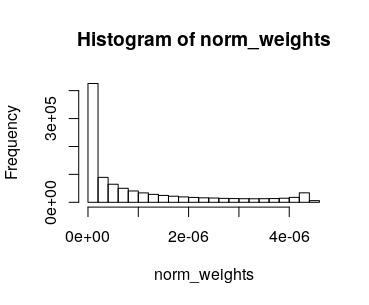
\includegraphics[width=100mm]{is_weights.png}
\end{center}

\end{frame}


%----------------------------------------------------------------------------------------
\begin{frame}[fragile]
\frametitle{Example 2}

Beware of bad proposal distributions!
\newline

A sample estimator of this approximate variance is
\[
\sum_{s=1}^s w(\theta^s) \left( h(\theta^s) - \hat{E}[h(\theta)]  \right)^2
\]
where $\hat{E}[h(\theta)] = \sum_s w(\theta^s)h(\theta^s)$. 
\newline

Note the weights aren't uniform like a ``standard" estimation of the sample variance.

\end{frame}

%----------------------------------------------------------------------------------------
\begin{frame}[fragile]
\frametitle{Example 2}

\begin{verbatim}
y <- 2 # fake data
log_unnorm_weight <- function(theta){ 
  # sqrt(2pi) because it will cancel out 
  -.5*(y - theta)^2 }
getISEstimator <- function(num_samples){
  theta_draws <- rt(num_samples , 1)
  lunws <- log_unnorm_weight(theta_draws)
  norm_weights <- exp(lunws)/sum(exp(lunws))
  estimator <- sum(norm_weights * theta_draws)
  list("estimate" = estimator, 
       "approx_var" = sum( norm_weights*(theta_draws - estimator)^2) ) }
# two ways to calculate standard errors
num_samps_per_estimate <- 10
sqrt(getISEstimator(num_samps_per_estimate)$approx_var)  
sd(replicate(1000, 
    getISEstimator(num_samps_per_estimate)$estimate)) 
\end{verbatim}


\end{frame}



\end{document} 


